% Begin the document and set up the style of the document
\documentclass[a4paper,11pt]{article}

% Install the required packages for the document 
\usepackage{enumitem}
\usepackage{amsmath}
\usepackage{amssymb}
\usepackage{verbatim}
\usepackage{mathtools}
\usepackage{tikz}
\usepackage{nicefrac}
\usepackage{bm}
\usepackage{xlop}

\newcommand{\norm}[1]{\left\lVert#1\right\rVert}


% Page and style settings
%\parskip=8pt
\parindent=0pt
% Right margin
\textwidth=6.25in
% Left margin
\oddsidemargin=0pt
\evensidemargin=0pt
% Bottom margin
\textheight=10in
% Top margin
\topmargin=-0.75in
\baselineskip=11pt
% end of page and other style settings

\renewcommand{\familydefault}{\sfdefault}
\usepackage{calrsfs}
\DeclareMathAlphabet{\pazocal}{OMS}{zplm}{m}{n}

\newcommand{\indep}{\mathrel{\text{\scalebox{1.07}{$\perp\mkern-10mu\perp$}}}}
\newcommand{\p}{\mathbb{P}}
\newcommand{\e}{\mathbb{E}}
\newcommand{\ds}{\displaystyle}
\newcommand{\code}{\texttt}
\newcommand{\HRule}{\rule{\linewidth}{0.5mm}} % Defines a new command for the horizontal lines, change thickness here

\newenvironment{nscentre}
 {\parskip=0pt\par\nopagebreak\centering}
 {\par\noindent\ignorespacesafterend}


\usepackage{fullpage}

\usepackage{titlesec} % Used to customize the \section command
\titleformat{\section}{\bf}{}{0em}{}[\titlerule] % Text formatting of sections
\titlespacing*{\section}{0pt}{3pt}{3pt} % Spacing around sections

\begin{document}
\setlength{\abovedisplayskip}{8pt}{%
\setlength{\belowdisplayskip}{8pt}{%


\text{LSA}
\hfill
\text{University of Michigan}

\begin{nscentre}
	\textbf{MATH562: Continuous Optimisation}\\
	\textbf{Homework 4}\\
\end{nscentre}

\text{Name: Keegan Gyoery}
\hfill
\text{UM-ID: 31799451}

\pagenumbering{arabic}
	\begin{enumerate}[leftmargin=*]
		\item Consider the function $\ds{f(\mathbf{x}) = 2x_1^2-2x_1x_2+x_2^2+2x_1-2x_2}$, with the Steepest Descent method applied, and a sequence $\ds{\mathbf{x}^k}$. 
			\begin{enumerate}[label=\alph*)]
				\item If $\ds{\mathbf{x}^{2k+1} = \left(0,1-\frac{1}{5^k}\right)^T}$, applying two steps of Cauchy's Steepest Descent method, we are required to show that $\ds{\mathbf{x}^{2k+3} = \left(0,1-\frac{1}{5^{k+1}}\right)^T}$. Firstly, the gradient of $\ds{f(\mathbf{x}}$ is
					\begin{align*}
						\nabla f(\mathbf{x}) & = (4x_1-2x_2+2,\:-2x_1+2x_2-2)^T.
					\end{align*}
					So, substituting in $\ds{\mathbf{x}^{2k+1} = \left(0,1-\frac{1}{5^k}\right)^T}$, we have,
					\begin{align*}
						\therefore \nabla f(\mathbf{x}^{2k+1}) & = \left(2-2\left(1-\frac{1}{5^k}\right), \: 2\left(1-\frac{1}{5^k}\right)-2\right)^T \\
															   & = \left(\frac{2}{5^k}, \:-\frac{2}{5^k}\right)^T.
					\end{align*}
					This gives us $\ds{\mathbf{d}^{2k+1} = \left(\frac{2}{5^k}, \:-\frac{2}{5^k}\right)^T}$. Clearly, we have,
					\begin{align*}
						\mathbf{x}^{2k+1} + \theta \mathbf{d}^{2k+1} & = \left(-\frac{2\theta}{5^k}, \:\frac{5^k+2\theta -1}{5^k}\right)^T.
					\end{align*}
					Consider now $\ds{f\left(\mathbf{x}^{2k+1} + \theta \mathbf{d}^{2k+1}\right)}$,
					\begin{align*}
						f\left(\mathbf{x}^{2k+1} + \theta \mathbf{d}^{2k+1}\right) & = 2\left(-\frac{2\theta}{5^k}\right)^2 - 2\left(-\frac{2\theta}{5^k}\right)\left(\frac{5^k+2\theta -1}{5^k}\right) + \left(\frac{5^k+2\theta -1}{5^k}\right)^2\\
																			   &\phantom{{}={}} + 2\left(-\frac{2\theta}{5^k}\right) - 2\left(\frac{5^k+2\theta -1}{5^k}\right)\\
																			   & = \frac{20}{5^{2k}}\theta^2 -\frac{8}{5^{2k}}\theta + \frac{1}{5^{2k}} \\
						\therefore \frac{df\left(\mathbf{x}^{2k+1} + \theta \mathbf{d}^{2k+1}\right)}{d\theta} & = \frac{40}{5^{2k}}\theta -\frac{8}{5^{2k}}.
					\end{align*}
					Setting the derivative to 0 to find the minimum, we have,
					\begin{align*}
						\frac{df\left(\mathbf{x}^{2k+1} + \theta \mathbf{d}^{2k+1}\right)}{d\theta} & = 0 \\
						\therefore \frac{40}{5^{2k}}\theta -\frac{8}{5^{2k}} & = 0 \\
						\therefore \theta_{2k+1} & = \frac{1}{5}. \\
						\therefore \mathbf{x}^{2k+2} & = \mathbf{x}^{2k+1} + \theta_{2k+1} \mathbf{d}^{2k+1} \\
													 & = \left(-\frac{2}{5^{k+1}}, \:1-\frac{3}{5^{k+1}}\right)^T.
					\end{align*}
					Applying the next iteration of the Steepest Descent Method, we have 
					\begin{align*}
						\therefore \nabla f(\mathbf{x}^{2k+2}) & = \left(-\frac{8}{5^{k+1}}-2 + \frac{6}{5^{k+1}} + 2, \: \frac{4}{5^{k+1}} + 2 - \frac{6}{5^{k+1}} - 2\right)^T \\
															   & = \left(-\frac{2}{5^{k+1}}, \:-\frac{2}{5^{k+1}}\right)^T.
					\end{align*}
					This gives us $\ds{\mathbf{d}^{2k+2} = \left(\frac{2}{5^{k+1}}, \:\frac{2}{5^{k+1}}\right)^T}$. Clearly, we have,
					\begin{align*}
						\mathbf{x}^{2k+2} + \theta \mathbf{d}^{2k+2} & = \left(\frac{2\theta-2}{5^{k+1}}, \:\frac{5^{k+1}+2\theta -3}{5^{k+1}}\right)^T.
					\end{align*}
					Consider now $\ds{f\left(\mathbf{x}^{2k+2} + \theta \mathbf{d}^{2k+2}\right)}$,
					\begin{align*}
						f\left(\mathbf{x}^{2k+2} + \theta \mathbf{d}^{2k+2}\right) & = 2\left(\frac{2\theta-2}{5^{k+1}}\right)^2 - 2\left(\frac{2\theta-2}{5^{k+1}}\right)\left(\frac{5^{k+1}+2\theta -3}{5^{k+1}}\right) \\
							&\phantom{{}={}}+ \left(\frac{5^{k+1}+2\theta -3}{5^{k+1}}\right)^2 + 2\left(\frac{2\theta-2}{5^{k+1}}\right) - 2\left(\frac{5^{k+1}+2\theta -3}{5^{k+1}}\right)\\
																			   & = \frac{4}{5^{2k+2}}\theta^2 -\frac{8}{5^{2k+2}}\theta + \frac{1}{5^{2k+2}}-1 \\
						\therefore \frac{df\left(\mathbf{x}^{2k+1} + \theta \mathbf{d}^{2k+1}\right)}{d\theta} & = \frac{8}{5^{2+2k}}\theta -\frac{8}{5^{2k+2}}.
					\end{align*}
					Setting the derivative to 0 to find the minimum, we have,
					\begin{align*}
						\frac{df\left(\mathbf{x}^{2k+1} + \theta \mathbf{d}^{2k+1}\right)}{d\theta} & = 0 \\
						\therefore \frac{8}{5^{2+2k}}\theta -\frac{8}{5^{2k+2}} & = 0 \\
						\therefore \theta_{2k+2} & = 1. \\
						\therefore \mathbf{x}^{2k+3} & = \mathbf{x}^{2k+2} + \theta_{2k+2} \mathbf{d}^{2k+2} \\
													 & = \left(0, \:1-\frac{1}{5^{k+1}}\right)^T.
					\end{align*}

				\item As seen in the included images, the Steepest Descent Method starting at $\ds{\mathbf{x}^1 = \mathbf{0}}$ zig-zags towards the minimum, located at $\ds{(0,1)^T}$. Note that consecutive descent directions are perpendicular, a fact we will prove later in the assignment.
					\pagebreak
					\begin{figure}[!ht]
						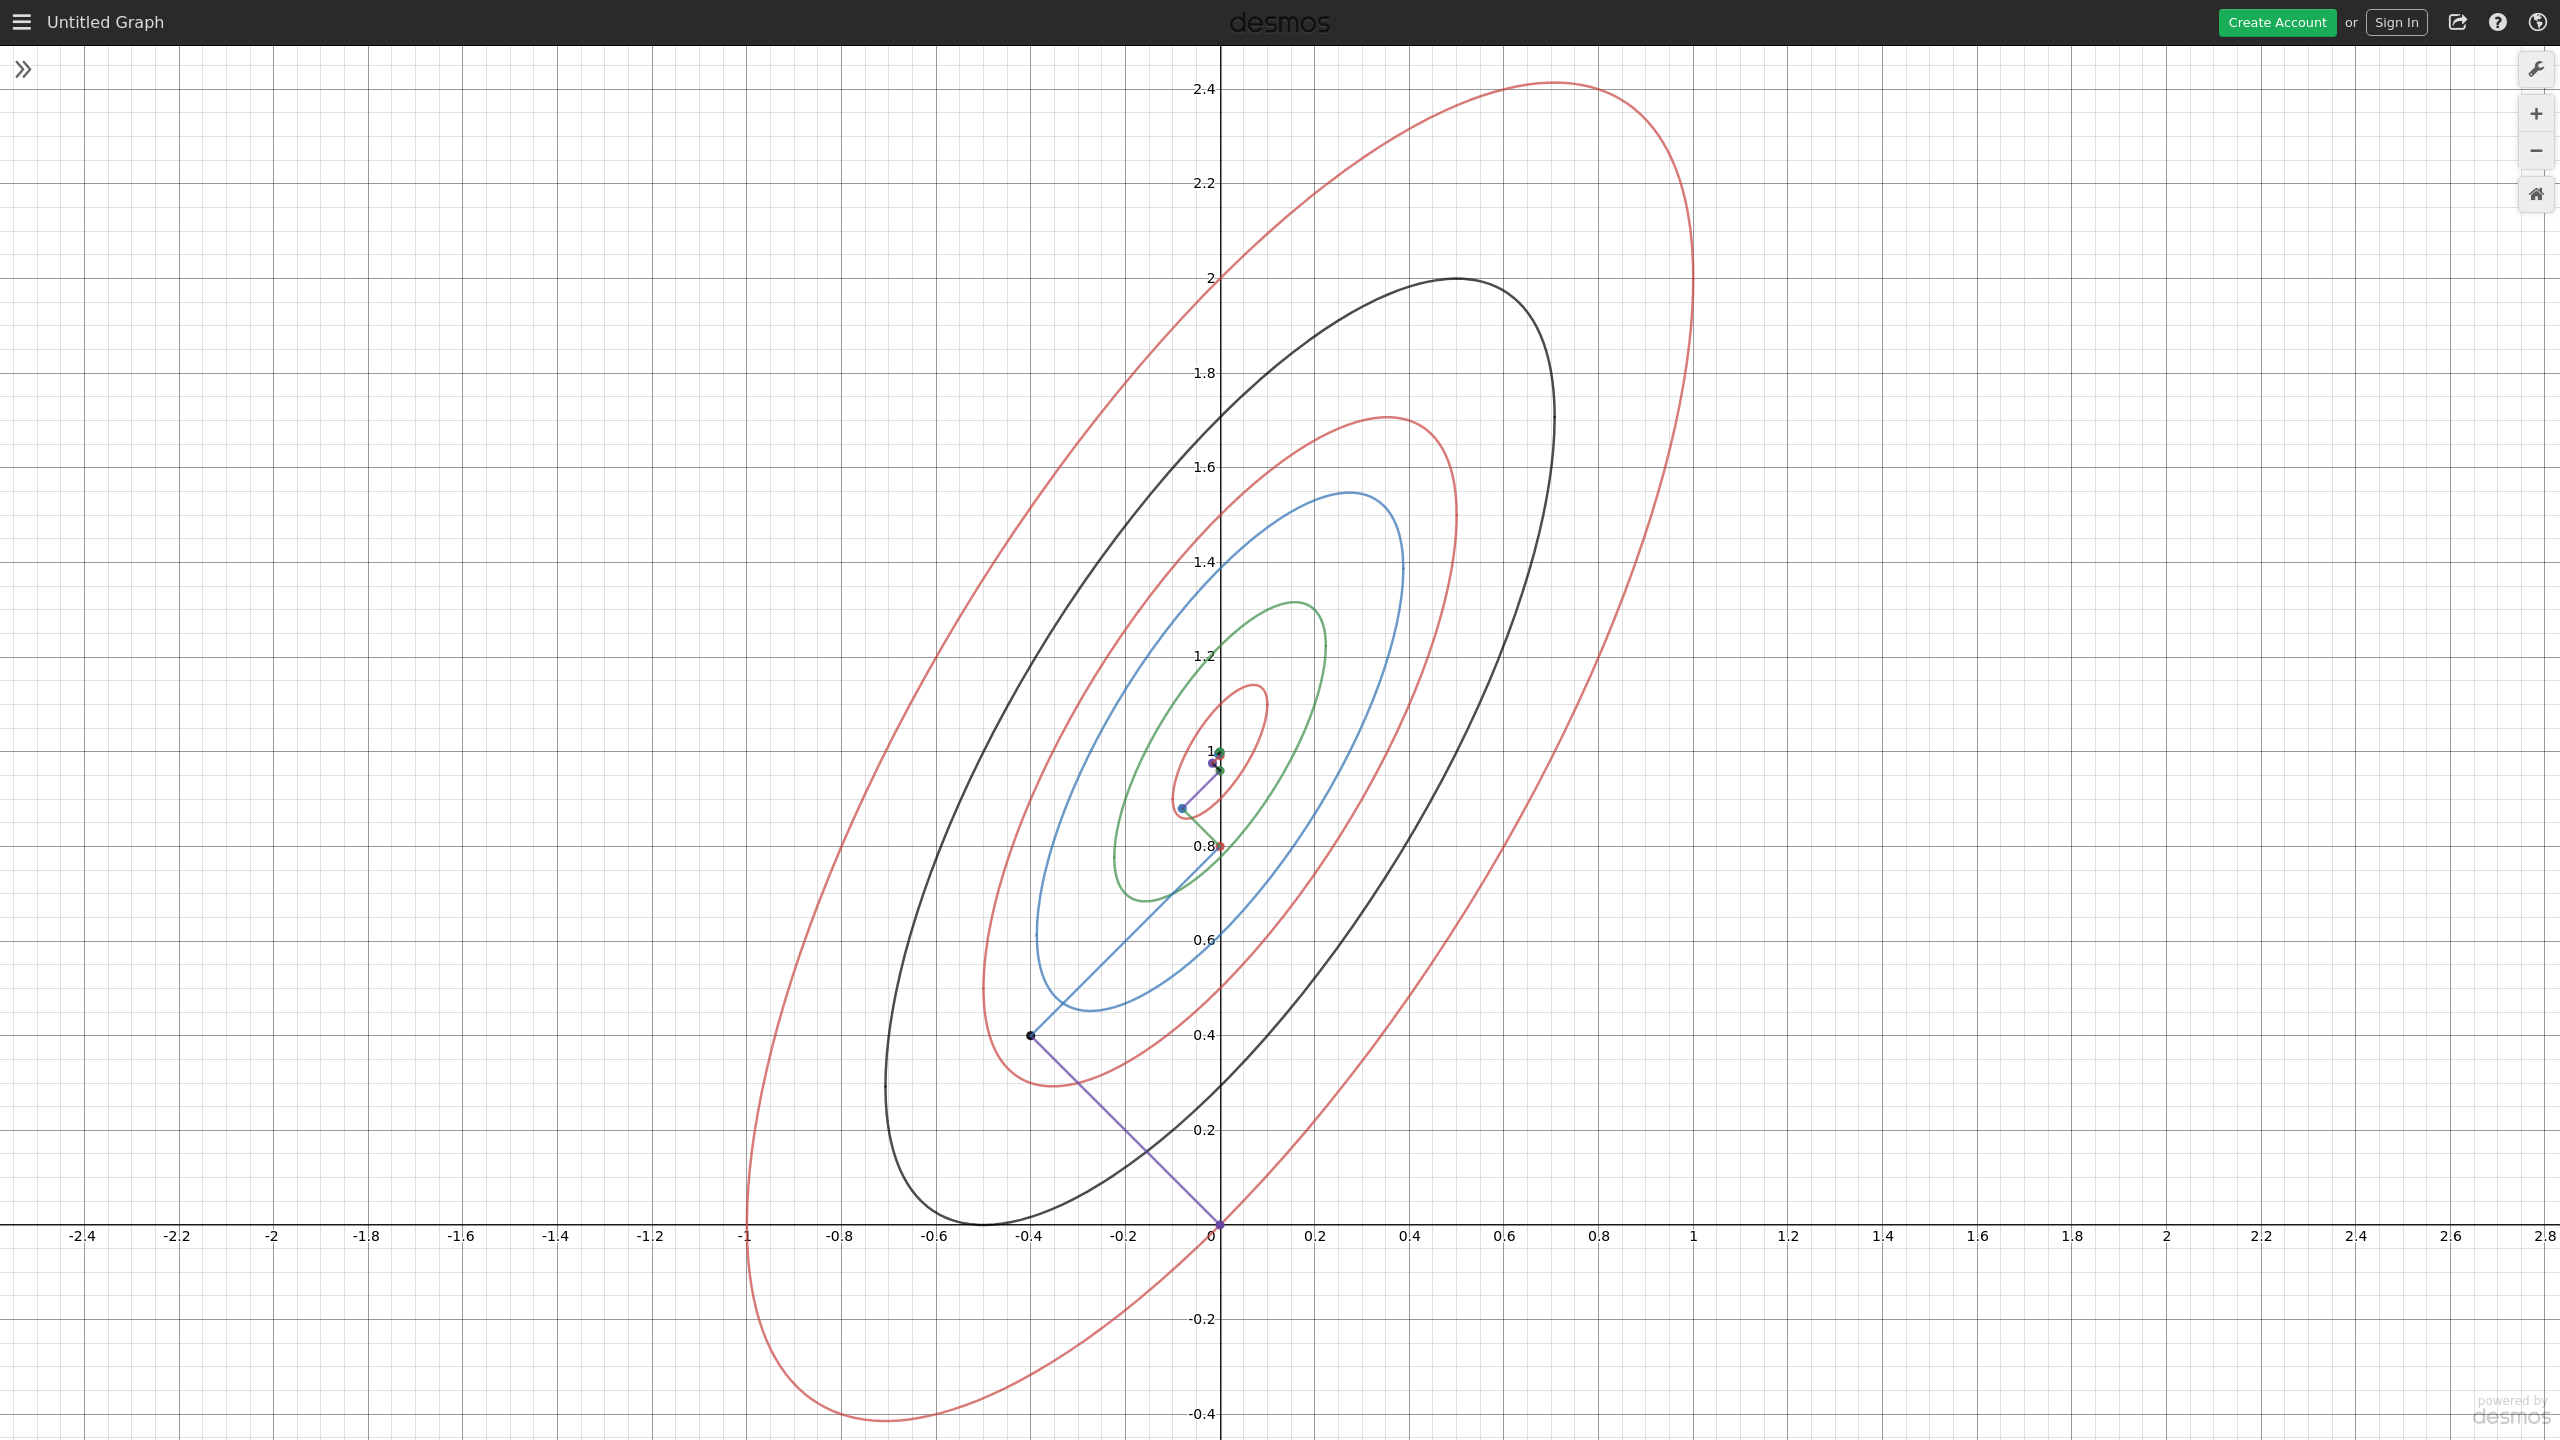
\includegraphics[width=\linewidth]{plane.png}
					\end{figure}
					\begin{figure}[!ht]
						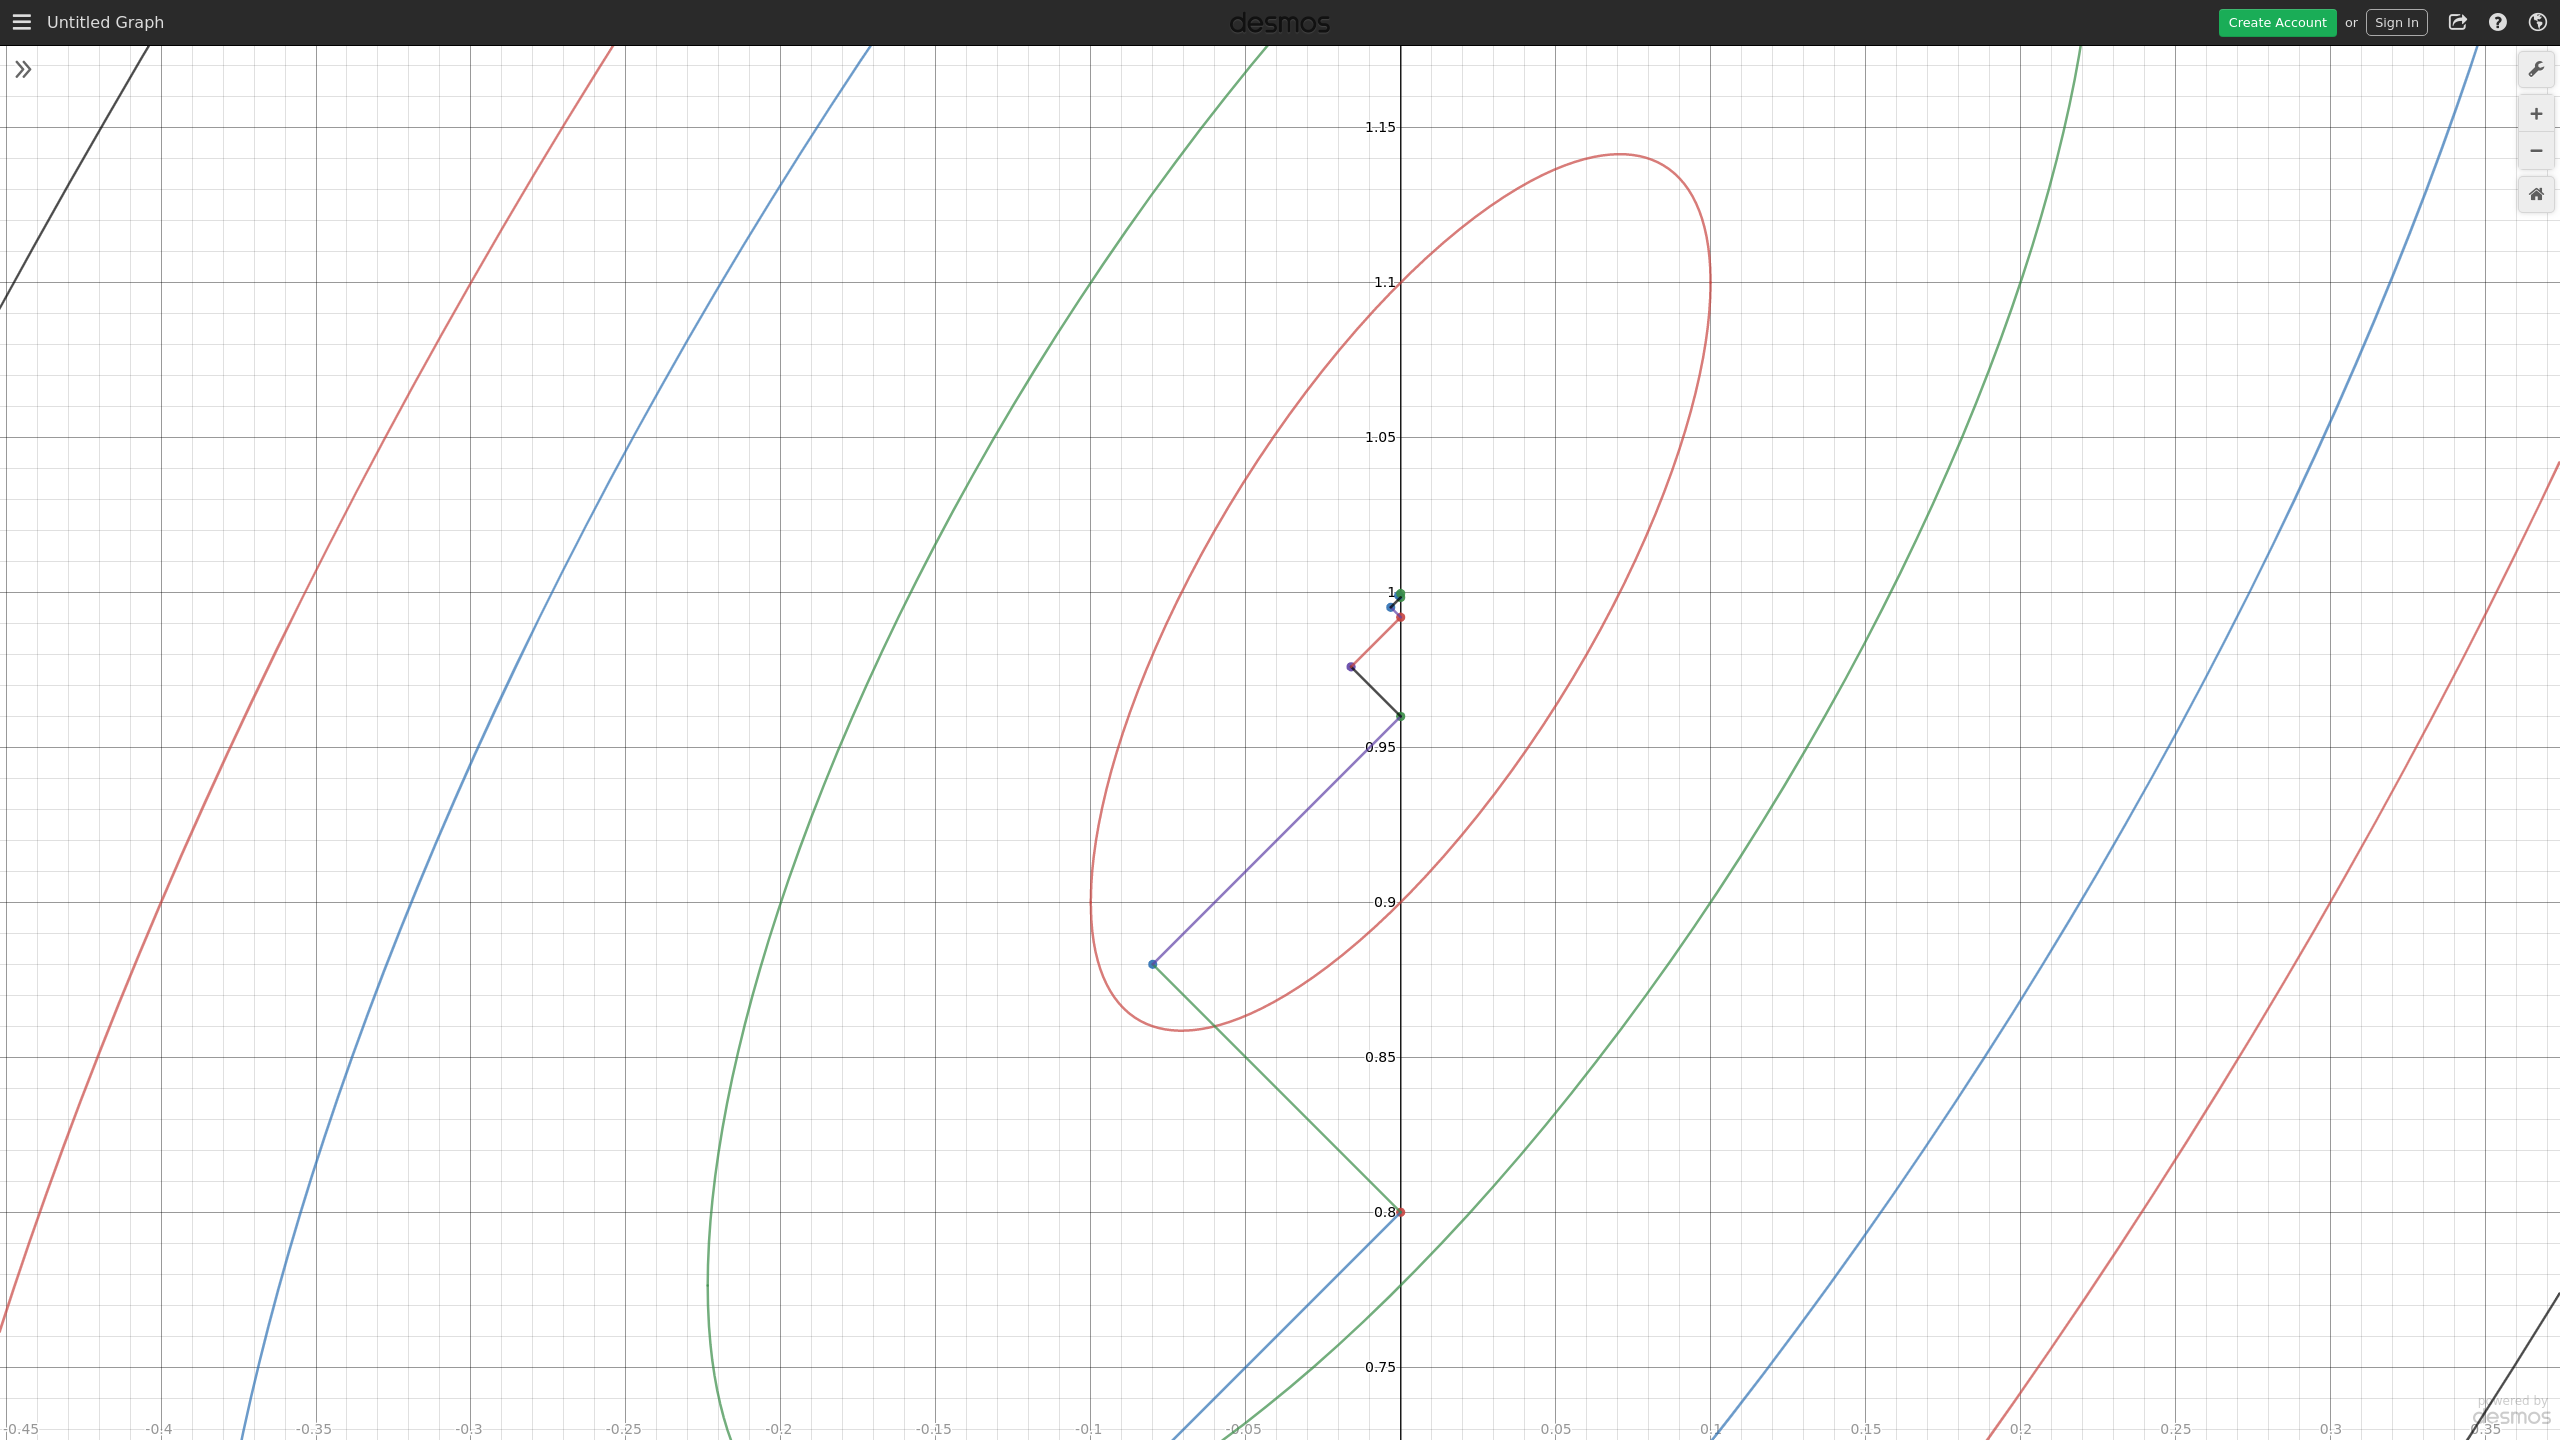
\includegraphics[width=\linewidth]{zoom.png}
					\end{figure}
					

			\end{enumerate}
			\pagebreak
		\item Assuming that $\ds{\mathbf{x}^k}$ and $\ds{\mathbf{x}^{k+1}}$ are consecutive points generated by the Steepest Descent Method, we have by defintion,
			\begin{align*}
				\frac{df\left(\mathbf{x}^{k} + \theta \mathbf{d}^{k}\right)}{d\theta}\bigg|_{\theta=\theta_k} & = 0 \\
				\therefore \nabla f\left(\mathbf{x}^{k} + \theta \mathbf{d}^{k}\right)^T\mathbf{d}^k\Big|_{\theta=\theta_k} & = 0 \\
				\therefore \nabla f\left(\mathbf{x}^{k} + \theta \mathbf{d}^{k}\right)^T\Big|_{\theta=\theta_k}\mathbf{d}^k & = 0 \\
				\therefore \nabla f\left(\mathbf{x}^{k+1} \right)^T\mathbf{d}^k & = 0 \\
				\therefore \left(-\mathbf{d}^{k+1} \right)^T\mathbf{d}^k & = 0 \\
				\therefore \left(\mathbf{d}^{k+1} \right)^T\mathbf{d}^k & = 0.
			\end{align*}
			Thus, the dot product of $\ds{\mathbf{d}^k}$ and $\ds{\mathbf{d}^{k+1}}$ is 0, and so the descent directions of consecutive points are orthogonal.
		\item Consider the function $\ds{f(\mathbf{x}) = \left(x_1^2-x_2\right)^2 + 2\left(x_2^2-x_1-4\right)^4}$ with $\ds{\mathbf{x}^0 = (2,1)^T}$.
			\begin{enumerate}[label=\alph*)]
				\item The gradient of $\ds{f(\mathbf{x})}$ is given by,
					\begin{align*}
						\nabla f(\mathbf{x}) & = 
						\begin{bmatrix}
							4x_1\left(x_1^2-x_2\right) - 8\left(x_2^2-x_1-4\right)^3 \\
							-2\left(x_1^2-x_2\right) + 16x_2\left(x_2^2-x_1-4\right)^3\\
						\end{bmatrix}, \\
						\therefore \nabla f(\mathbf{x}^0) & = (1024,-2006)^T.
					\end{align*}
				\item This gives us $\ds{\mathbf{d}^0 = (-1024, 2006)^T}$. Clearly, we have, $\ds{\mathbf{x}^{0} + \theta \mathbf{d}^{0} = (2-1024\theta, 1+2006\theta)^T}$. Now considering $\ds{a(\theta) = f(\mathbf{x}^{0} + \theta \mathbf{d}^{0})}$, 
					\begin{align*}
						a(\theta) & = f(\mathbf{x}^{0} + \theta \mathbf{d}^{0}) \\
								  & = f(2-1024\theta, 1+2006\theta) \\
						\therefore a(\theta) & = \left[(2-1024\theta)^2 - (1+2006\theta)\right]^2 + 2\left[(1+2006\theta)^2 - (2-1024\theta) - 4\right]^4 \\
					\end{align*}
				\item From $\ds{a(\theta)}$ above, we calculate the derivative as
					\begin{align*}
						a(\theta) & = \left[(2-1024\theta)^2 - (1+2006\theta)\right]^2 + 2\left[(1+2006\theta)^2 - (2-1024\theta) - 4\right]^4 \\
						\therefore a^{\prime}(\theta) & = 2\left[2(-1024)(2-1024\theta)-2006\right] \left[(2-1024\theta)^2 - (1+2006\theta)\right]\\
													  &\phantom{{}={}} + 2\times4\left[2\times2006(1+2006\theta)+1024\right]\left[(1+2006\theta)^2 - (2-1024\theta) - 4\right]^3 \\
						\therefore a^{\prime}(0) & = 2\left[2(-1024)\times 2 -2006\right] \left[(2)^2 - (1)\right] + 2\times4\left[2\times2006+1024\right]\left[(1)^2 - (2) - 4\right]^3 \\
												 & = (-12204) \times 3 + 40288\times (-125) \\
												 & = -5072612 \\
						\therefore a^{\prime}(\theta) < 0.
					\end{align*}
				\item Let $\ds{\beta = 1}$. Consider $\ds{a^{\prime}(\beta)}$.
					\begin{align*}
						a^{\prime}(\beta) & = a^{\prime}(1) \\
										  & = 2\left[2(-1024)(2-1024)-2006\right] \left[(2-1024)^2 - (1+2006)\right]\\
										  &\phantom{{}={}} + 2\times4\left[2\times2006(1+2006)+1024\right]\left[(1+2006)^2 - (2-1024) - 4\right]^3 \\
										  & \approx 4.21 \times 10^{27} \\
						\therefore a^{\prime}(\beta) & > 0.
					\end{align*}


				\item The code prints out the necessary variables to track, and may be viewed when run.
				\item The code prints out the necessary variables to track, and may be viewed when run.
				\item Using the MATLAB code for the golden section method, and with a smaller epsilon, we obtain  $\ds{\theta_0 = 0.0006}$. Thus, using $\ds{\mathbf{x}^0 = (2,1)^T}$ and $\ds{\mathbf{d}^0 = (-1024, 2006)^T}$, applying the one step of Steepest Descent Method gives us
					\begin{align*}
						\mathbf{x}^{1} & = \mathbf{x}^{0} + \theta_{0} \mathbf{d}^{0} \\
									   & = \left(1.3856,2.2036\right)^T.
					\end{align*}
			\end{enumerate}
	\end{enumerate}
\end{document}
